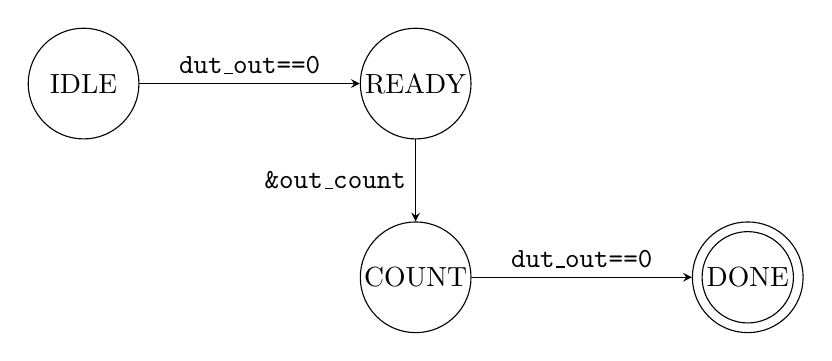
\begin{tikzpicture}
  [
    x=1em, y=1em,
    node/.style =
      {draw, circle, align=center, inner sep=0pt, minimum size=4em},
    sarrow/.style =
      { ->, >=stealth, font=\ttfamily}
  ]
  \node [node] at ( 0, 7)  (i) {IDLE};
  \node [node] at (12, 7) (r) {READY};
  \node [node] at (12, 0)  (c) {COUNT};
  \node [node] at (24, 0)  (d) {DONE};
  \node [draw, circle, inner sep=0pt, minimum size=3.3em] at (24, 0)  (dd) {};

  \draw [sarrow] (i.east)  -- node[above] {dut\_out==0}  (r.west);
  \draw [sarrow] (r.south) -- node[left]  {\&out\_count} (c.north);
  \draw [sarrow] (c.east)  -- node[above] {dut\_out==0}  (d.west);
\end{tikzpicture}